\documentclass[journal,transmag]{IEEEtran}

\usepackage{cite}
\usepackage[pdftex]{graphicx}
% declare the path(s) where your graphic files are
\graphicspath{reports/images/}
\DeclareGraphicsExtensions{.pdf,.jpeg,.png,.jpg}
\usepackage{amsmath}
\interdisplaylinepenalty=2500
\usepackage{algorithmic}
\usepackage{array}
\usepackage[caption=false,font=normalsize,labelfont=sf,textfon =sf]{subfig}
\usepackage{dblfloatfix}
\usepackage{url}
\usepackage{xcolor}
\usepackage{listings}

\lstset{
	escapeinside={/*@}{@*/},
	language=Java,	
	basicstyle=\fontsize{8.5}{12}\selectfont,
	numbers=left,
	numbersep=2pt,    
	xleftmargin=2pt,
	frame=tb,
	columns=fullflexible,
	showstringspaces=false,
	tabsize=4,
	keepspaces=true,
	showtabs=false,
	showspaces=false,
	morekeywords={inline,public,class,private,protected,struct},
	captionpos=b,
	lineskip=-0.4em,
	aboveskip=10pt,
	extendedchars=true,
	breaklines=true,
	prebreak = \raisebox{0ex}[0ex][0ex]{\ensuremath{\hookleftarrow}},
	keywordstyle=\color[rgb]{0,0,1},
	commentstyle=\color[rgb]{0.133,0.545,0.133},
	stringstyle=\color[rgb]{0.627,0.126,0.941},
}

% correct bad hyphenation here
\hyphenation{hy-phen}

\begin{document}
    \title{Concurrent and Parallel Systems: Coursework 2 Report}
    \author{
        \IEEEauthorblockN{Gareth Pulham, 40099603}
        \IEEEauthorblockA{School of Computing, Edinburgh Napier University, Edinburgh}
    }
    \IEEEtitleabstractindextext{
        \begin{abstract}
            As part of Napier University's Concurrent and Parallel Systems class (SET10108), students were tasked to
            investigate and parallelise where possible one of three example problems. This document will cover one such
            investigation, covering how an N-body simulation was initially developed in a sequential fashion and then
            parallelised on a GPU.
        \end{abstract}
    }

    \maketitle
    \IEEEdisplaynontitleabstractindextext

    \section{Introduction}
    This report aims to implement and investigate the performance of a sequential N-body simulation, and to evaluate
    the improvement that can be seen when converting the simulation to a parallelised solution, in this instance via
    GPU parallelisation.

        \subsection{Introduction to N-body simulations}
        N-body simulations are simulations of physical systems of bodies, such as planets or stars, and how they move
        in relation to each other under the gravitational (or other, for example, electrostratic) forces acted on each
        other. These simulations are useful in the fields of astronomy and physics, where they can model
        computationally, and thus more easily measurable, interactions that may not be easily measurable in real life.
        Additionally, by varying simulation parameters, they can be used to simulate the passage of time at much higher
        rates than appear in nature, allowing the simulation and visualisation of systems of bodies as they progress
        years into the future in much shorter time scales.

        Naive N-body simulations are very simple programs, however, they are computationally hard. A variety of ways to
        reduce the computational load, and speed up simulations exist, however, they rely on approximation.

        At its simplest, an N-body simulation simply iterates over all bodies in the system and for each, accumulates
        the force applied to it by all others \cite{frans}. In essence:

        \begin{algorithmic}
            \FORALL{thisbody in bodies}
                \STATE $ \vec{f} = 0 $
                \FORALL{otherbody in bodies}
                    \STATE $ \vec{f} = \vec{f} + force(thisbody, otherbody) $
                \ENDFOR
                \STATE $ accelerate(thisbody, \vec{f}) $
            \ENDFOR
        \end{algorithmic}

        where $ force() $ calculates the force vector applied by $ otherbody $ on $ thisbody $, and $ accelerate() $
        calculates how the velocity of a body should change given a force vector. Then, for each body, the positions
        of each body are changed according to their velocity.

        This can be seen to be an $ n^2 $ problem for $ n $ bodies.

        \subsection{Introduction to GPU parallelisation}
        The computational architecture of modern GPUs were designed to best apply simple ``shader'' programs to an
        an entire image, a 2-dimensional array of colours. In time, it was recognised that these collections of compute
        cores, though slow and simple, are very well applied to problems with large amounts of data which can be
        operated on all at once.

        Due to the graphical history of GPU computing, these cores are typically considered a grid of processing cores
        that can be grouped into a collection of larger blocks executing in lockstep. These grids of processors have
        been made more available for general purpose computing with the development of parallel computing frameworks
        such as OpenCL \cite{OpenCL} and CUDA \cite{CUDA}, which expose consistent interfaces to execute work on GPUs from traditional
        CPU-based programs on the GPU host computer. By writing short, C-like programs, programmers can utilise
        compilers within these frameworks to compile, load, and execute ``kernels'', that operate over given data in
        parallel.

        \begin{figure}[h]
            \centering
            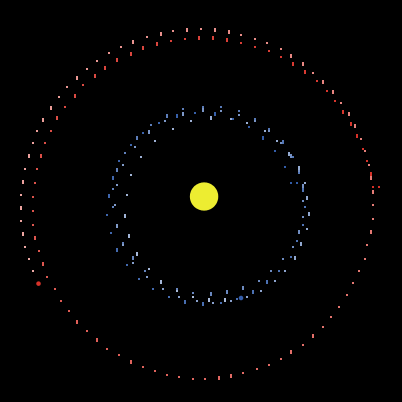
\includegraphics[width=0.5\textwidth]{report/images/nbody.png}
            \caption{N-body simulation. NetLogo, CC-BY-NC-SA. http://ccl.northwestern.edu/netlogo/models/N-Bodies}
        \end{figure}

        \subsection{Hardware}
        During the development and evaluation of both the serial and parallel N-body simulation, a single, consistent
        computing environment was used. The specification of this server follows:

        \begin{itemize}
            \item Intel(R) Core(TM) i7-4770K CPU @ 3.50GHz
            \item 8GB RAM
            \item 2x Nvidia Tesla K40c GPGPU cards
            \item Manjaro Linux 16.10 ``Fringilla''
        \end{itemize}

    \section{Methodology}
    Initially, time was spent researching the different methods and optimisations used to implement N-body simulations,
    such as tools for approximating small and remote clusters of bodies from the current body, like Barnes-Hut trees
    \cite{BarnesHut}.

    Ultimately, to best illustrate and investigate the difference between CPU and GPU approaches, a naive
    implementation that could be applied to both platforms with minimal changes was developed.

    Once the initial CPU implentation was written, a simple frontend was developed that could be run locally, allowing
    the simulation to be visualised. This was particularly useful as it allowed identification of any issues by
    observing how the simulation ran on an intuitive level and greatly sped up the process of identifying and
    correcting any bugs found in the implementation. For example, it was noted on the first run in the visual front end
    that instead of coming together, bodies in the system accelerated away from each other - this immediately signalled
    a sign error in the force calculation that was quickly corrected.

    \begin{figure}[h]
        \centering
        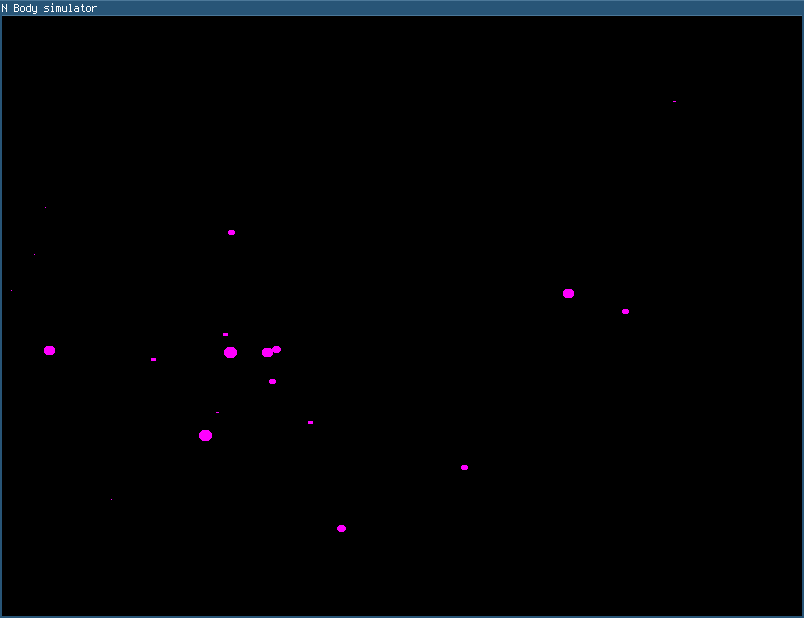
\includegraphics[width=0.5\textwidth]{report/images/nbody_vis.png}
        \caption{The N-body visualiser}
    \end{figure}

    Following the development and testing of the CPU solution, the next step was to port the simulation code into an
    OpenCL kernel. Due to keeping the GPU port in mind, this was a simple process with the kernel being almost a
    verbatim copy of the CPU simulation step code, notably, the main difference was decomposing the single complete
    \texttt{body} type in the CPU code (holding x/y position, velocity, etc) into a collection of arrays, as OpenCL
    kernels can not inherit compound types from the host.

    Again, to test the results of the implementation, steps were taken to allow the visualisation of the simulation.
    Because of the compute machine being ``headless'' (ie, without an accessible monitor), in this instance the state
    of the simulation was frequently dumped to file, which could then be played back locally.

    Following testing of the implementations, they were time for execution speed. Reasonably set simulation parameters
    were determined empirically, and set to 1024 bodies, running for 100000 iterations. The two implementations were
    then timed with simple timestamping code around the execution of the simulation, and run multiple times and the
    runtimes averaged.

    An additional tunable value in the GPU implementation is the workgroup size. This is the number of GPU cores
    operating together, and sharing memory. GPU simulation speeds across a range of workgroup sizes (from 1 to
    1024, in powers of 2) were tested.

    Once these results were gathered, they were compared. Of particular interest was the speedup between CPU and GPU
    implementations. The speedup is given as the ratio between sequential and parallelised implementations of the
    simulation: $ S = \frac{Sequential}{Parallel} $ .

    \section{Results}
        \subsection{Measurements}
        The execution times for the CPU implementation are as shown:
        \begin{table}[h]
            \centering
            \caption{CPU timings}
            \label{CPUTable}
            \begin{tabular}{ c c }
                Iteration & Time (s) \\
                \hline
                \hline
                1         & 1140 \\
                2         & 1144 \\
                3         & 1141 \\
                4         & 1143 \\
                5         & 1140 \\
                6         & 1141 \\
                7         & 1140 \\
                8         & 1140 \\
                9         & 1141 \\
                10        & 1140 \\
                \hline
                Average   & 1141 \\
            \end{tabular}
        \end{table}

        The execution times for the GPU implementation are as shown:
        \begin{table}[h]
            \centering
            \caption{GPU timings}
            \label{GPUTable}
            \begin{tabular}{ c c }
                Iteration & Time (s) \\
                \hline
                \hline
                1         & 167 \\
                2         & 167 \\
                3         & 167 \\
                4         & 168 \\
                5         & 167 \\
                6         & 167 \\
                7         & 167 \\
                8         & 167 \\
                9         & 167 \\
                10        & 167 \\
                \hline
                Average   & 167.1 \\
            \end{tabular}
        \end{table}

        The workgroup size was picked based on the following results:
        \begin{figure}[h]
            \centering
            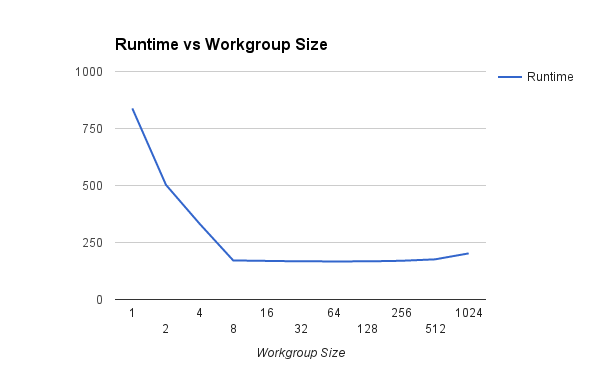
\includegraphics[width=0.5\textwidth]{report/images/RuntimeVsWorkgroupSize.png}
            \caption{Runtime vs Workgroup Size}
        \end{figure}

        \begin{table}[h]
            \centering
            \caption{GPU timings vs Group Size}
            \label{GPUvsGroupsSizeTable}
            \begin{tabular}{ c c }
                Group Size & Time (s) \\
                \hline
                \hline
                   1       & 838.2 \\
                   2       & 502.9 \\
                   4       & 332.3 \\
                   8       & 171.3 \\
                  16       & 169.3 \\
                  32       & 167.4 \\
                \hline
                  64       & 167.1 \\
                \hline
                 128       & 167.3 \\
                 256       & 169.8 \\
                 512       & 176.1 \\
                1024       & 202.2 \\
            \end{tabular}
        \end{table}

        \subsection{Results summary}
        From the above results, we see that for our given workload and kernel, performance peaks with 64-core
        workgroups. If we then compare the timings for this configuration with the CPU implementation, we can see a
        speedup of $ \frac{Sequential}{Parallel} = \frac{1141}{167.1} = 6.83\times $.

    \section{Conclusion}
    To conclude, this report covers an investigation of the N-body problem, particularly focussing on how GPUs can be
    used to parallelise the problem to affect a speedup. In doing so, the author developed both a CPU and a GPU
    implementation on the N-body problem of similar style and capability, focussing on minimal changes between versions
    to isolate what speedup can be brought about by the GPU compute paradigm. After recording and analysing the results,
    the author identified a speedup of almost $ 7\times $.

    Additionally, the author believes that the speedup can be further improved by including further changes to bring the
    simulation into line with GPU strengths, for example vectorisation of the force, acceleration, velocity and position
    properties of bodies within the simulation.

    \newpage

    \appendices
    \section{CPU execution time measurements}
    \begin{table}[h]
        \centering
        \caption{CPU timings}
        \label{CPUTableRaw}
        \begin{tabular}{ c c }
            Iteration & Time (s) \\
            \hline
            \hline
            1         & 1140 \\
            2         & 1144 \\
            3         & 1141 \\
            4         & 1143 \\
            5         & 1140 \\
            6         & 1141 \\
            7         & 1140 \\
            8         & 1140 \\
            9         & 1141 \\
            10        & 1140 \\
        \end{tabular}
    \end{table}

    \section{GPU execution time measurements}
     \begin{table}[h]
        \centering
        \caption{GPU timings}
        \label{GPUTableRaw}
        \begin{tabular}{ c c }
            Iteration & Time (s) \\
            \hline
            \hline
                1     & 167 \\
                2     & 167 \\
                3     & 167 \\
                4     & 168 \\
                5     & 167 \\
                6     & 167 \\
                7     & 167 \\
                8     & 167 \\
                9     & 167 \\
                10    & 167 \\
       \end{tabular}
    \end{table}

    \section{GPU execution time under varying workgroup size measurements}
    \begin{table}[h]
        \centering
        \caption{GPU timings under varying workgroup size}
        \label{GPUWorkGroupTableRaw}
        \begin{tabular}{ c c c c c c c c c c c c }
            Iteration &   1 &   2 &   4 &   8 &  16 &  32 &  64 & 128 & 256 & 512 & 1024 \\
            \hline
            \hline
             1        & 837 & 503 & 332 & 171 & 170 & 167 & 167 & 168 & 169 & 176 &  202 \\
             2        & 839 & 503 & 333 & 171 & 169 & 168 & 167 & 168 & 169 & 176 &  202 \\
             3        & 839 & 503 & 333 & 171 & 169 & 167 & 167 & 167 & 170 & 176 &  202 \\
             4        & 838 & 503 & 331 & 171 & 169 & 168 & 168 & 167 & 169 & 176 &  202 \\
             5        & 839 & 503 & 333 & 172 & 169 & 167 & 167 & 167 & 172 & 176 &  203 \\
             6        & 838 & 503 & 331 & 172 & 169 & 167 & 167 & 167 & 171 & 176 &  203 \\
             7        & 839 & 502 & 333 & 171 & 169 & 168 & 167 & 167 & 170 & 176 &  202 \\
             8        & 387 & 503 & 332 & 171 & 170 & 167 & 167 & 167 & 170 & 177 &  202 \\
             9        & 838 & 502 & 332 & 171 & 169 & 167 & 167 & 168 & 169 & 176 &  202 \\
            10        & 838 & 504 & 333 & 172 & 170 & 168 & 167 & 167 & 169 & 176 &  202 \\
        \end{tabular}
    \end{table}

    \bibliographystyle{IEEEtran}
    \bibliography{report}

\end{document}
